\documentclass[twocolumn]{article}

\usepackage[english]{babel} 


\usepackage[utf8]{inputenc}
\usepackage[T1]{fontenc}
\usepackage{lmodern}
\usepackage{amsmath}
\usepackage{verbatim}
\usepackage{amssymb}
\usepackage{mathtools}
\usepackage{enumitem}
\usepackage{float}
\usepackage{titlesec} 

\titleformat{\subsection}[runin]{\normalfont\large\bfseries}{\thesubsection}{1em}{}

\setlength{\parindent}{0pt}

\begin{document}

\begin{center}

\Large{\textbf{MLDS: Homework 4}} \\
\textsc{\large{Andraž De Luisa}} \\
\vspace{6pt}
\small{\today}

\end{center}

Implement kernelized ridge regression with two kernels: polynomial $\kappa (x, x') = (1 + x x')^M $ and RBF kernel: $\kappa (x, x') = \exp(- \frac{||x - x'||^2}{2 \sigma^2})$.

\subsection*{Task 1}

Figure \ref{fig:sine} shows the fitting of the kernelized ridge regression model on the sine dataset, with two different kernels: a polynomial and a RBF (radial basis function) kernel. The values of the kernel parameters are not optimal with respect to any measure, I have just chosen such values that visually fit well to the actual sine values from the data. A smaller value of the degree M in the polynomial kernel would result in a flattened curve, while a higher M would cause a clear overfit. A similar behaviour could be seen with the RBF kernel, with the lost of smoothness (i.\ e. overfit) for lower $\sigma$, and a flattening for higher ones.

\begin{figure}[ht]
    \centering
    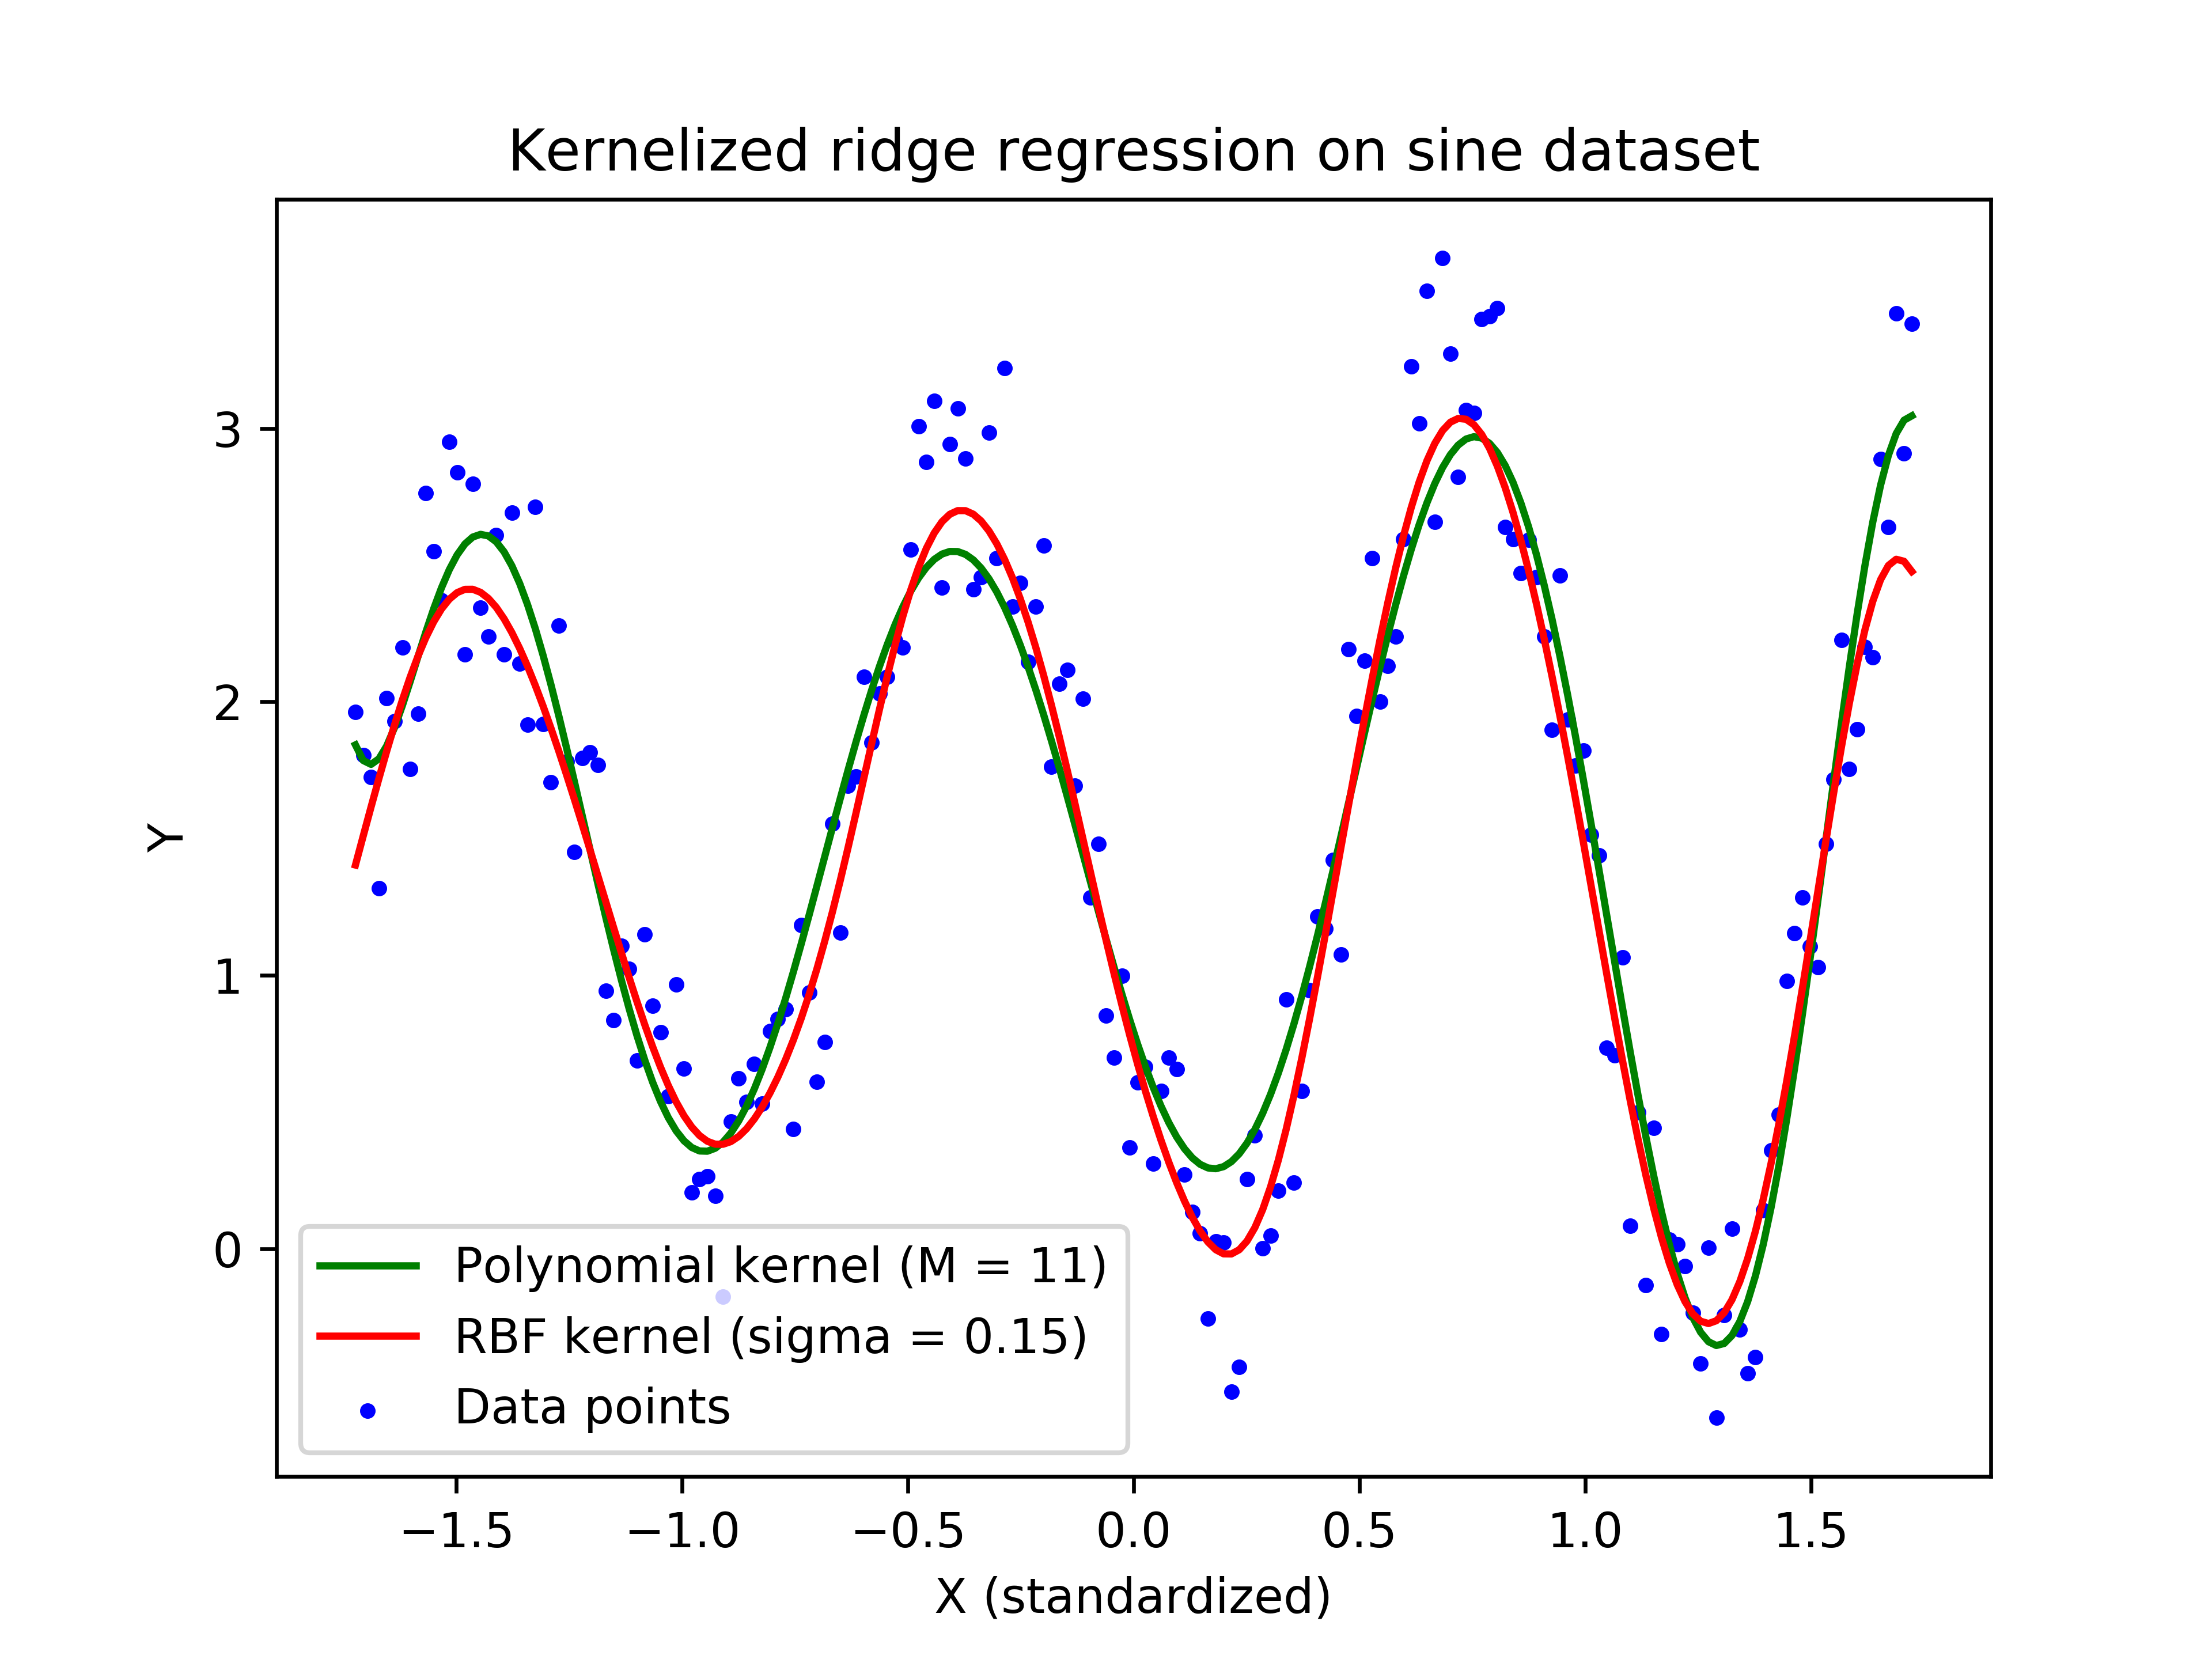
\includegraphics[width=.4\textwidth]{sine.png}
    \caption{Kernelized ridge regression with a polynomial and a RBF kernel, both with regularization parameter $\lambda = 1$. Note that values on the x axis are standardized for numerical stability reasons.}
    \label{fig:sine}
\end{figure}

\subsection*{Task 2}

Figures \ref{fig:house_pol} and \ref{fig:house_rbf} show the evaluation of the kernelized ridge regression with polynomial and RBF kernel on the test data from the housing dataset. As the measure of predictive performance the RMSE (rooted mean squared errors) was used, both in parameter optimization and model evaluation. Both figures present a comparison between a fixed regularization parameter $\lambda  = 1$ and the best $\lambda$ for each kernel parameter (M or $\sigma$), set with internal 10-fold cross-validation. In figure \ref{fig:house_pol} is clear how the performance decreases for degrees bigger than 4, which is caused by the overfit (the RMSE on the training data drops almost to 0). On the plot the higher degrees $M > 6$ are omitted on purpose for a nicer visualization. Similarly, we prefer higher $\sigma$-s in the RBF kernel as shown in figure \ref{fig:house_rbf}. For both cases we also see that the optimization of $\lambda$ with internal CV is useful.

\begin{figure}[ht]
    \centering
    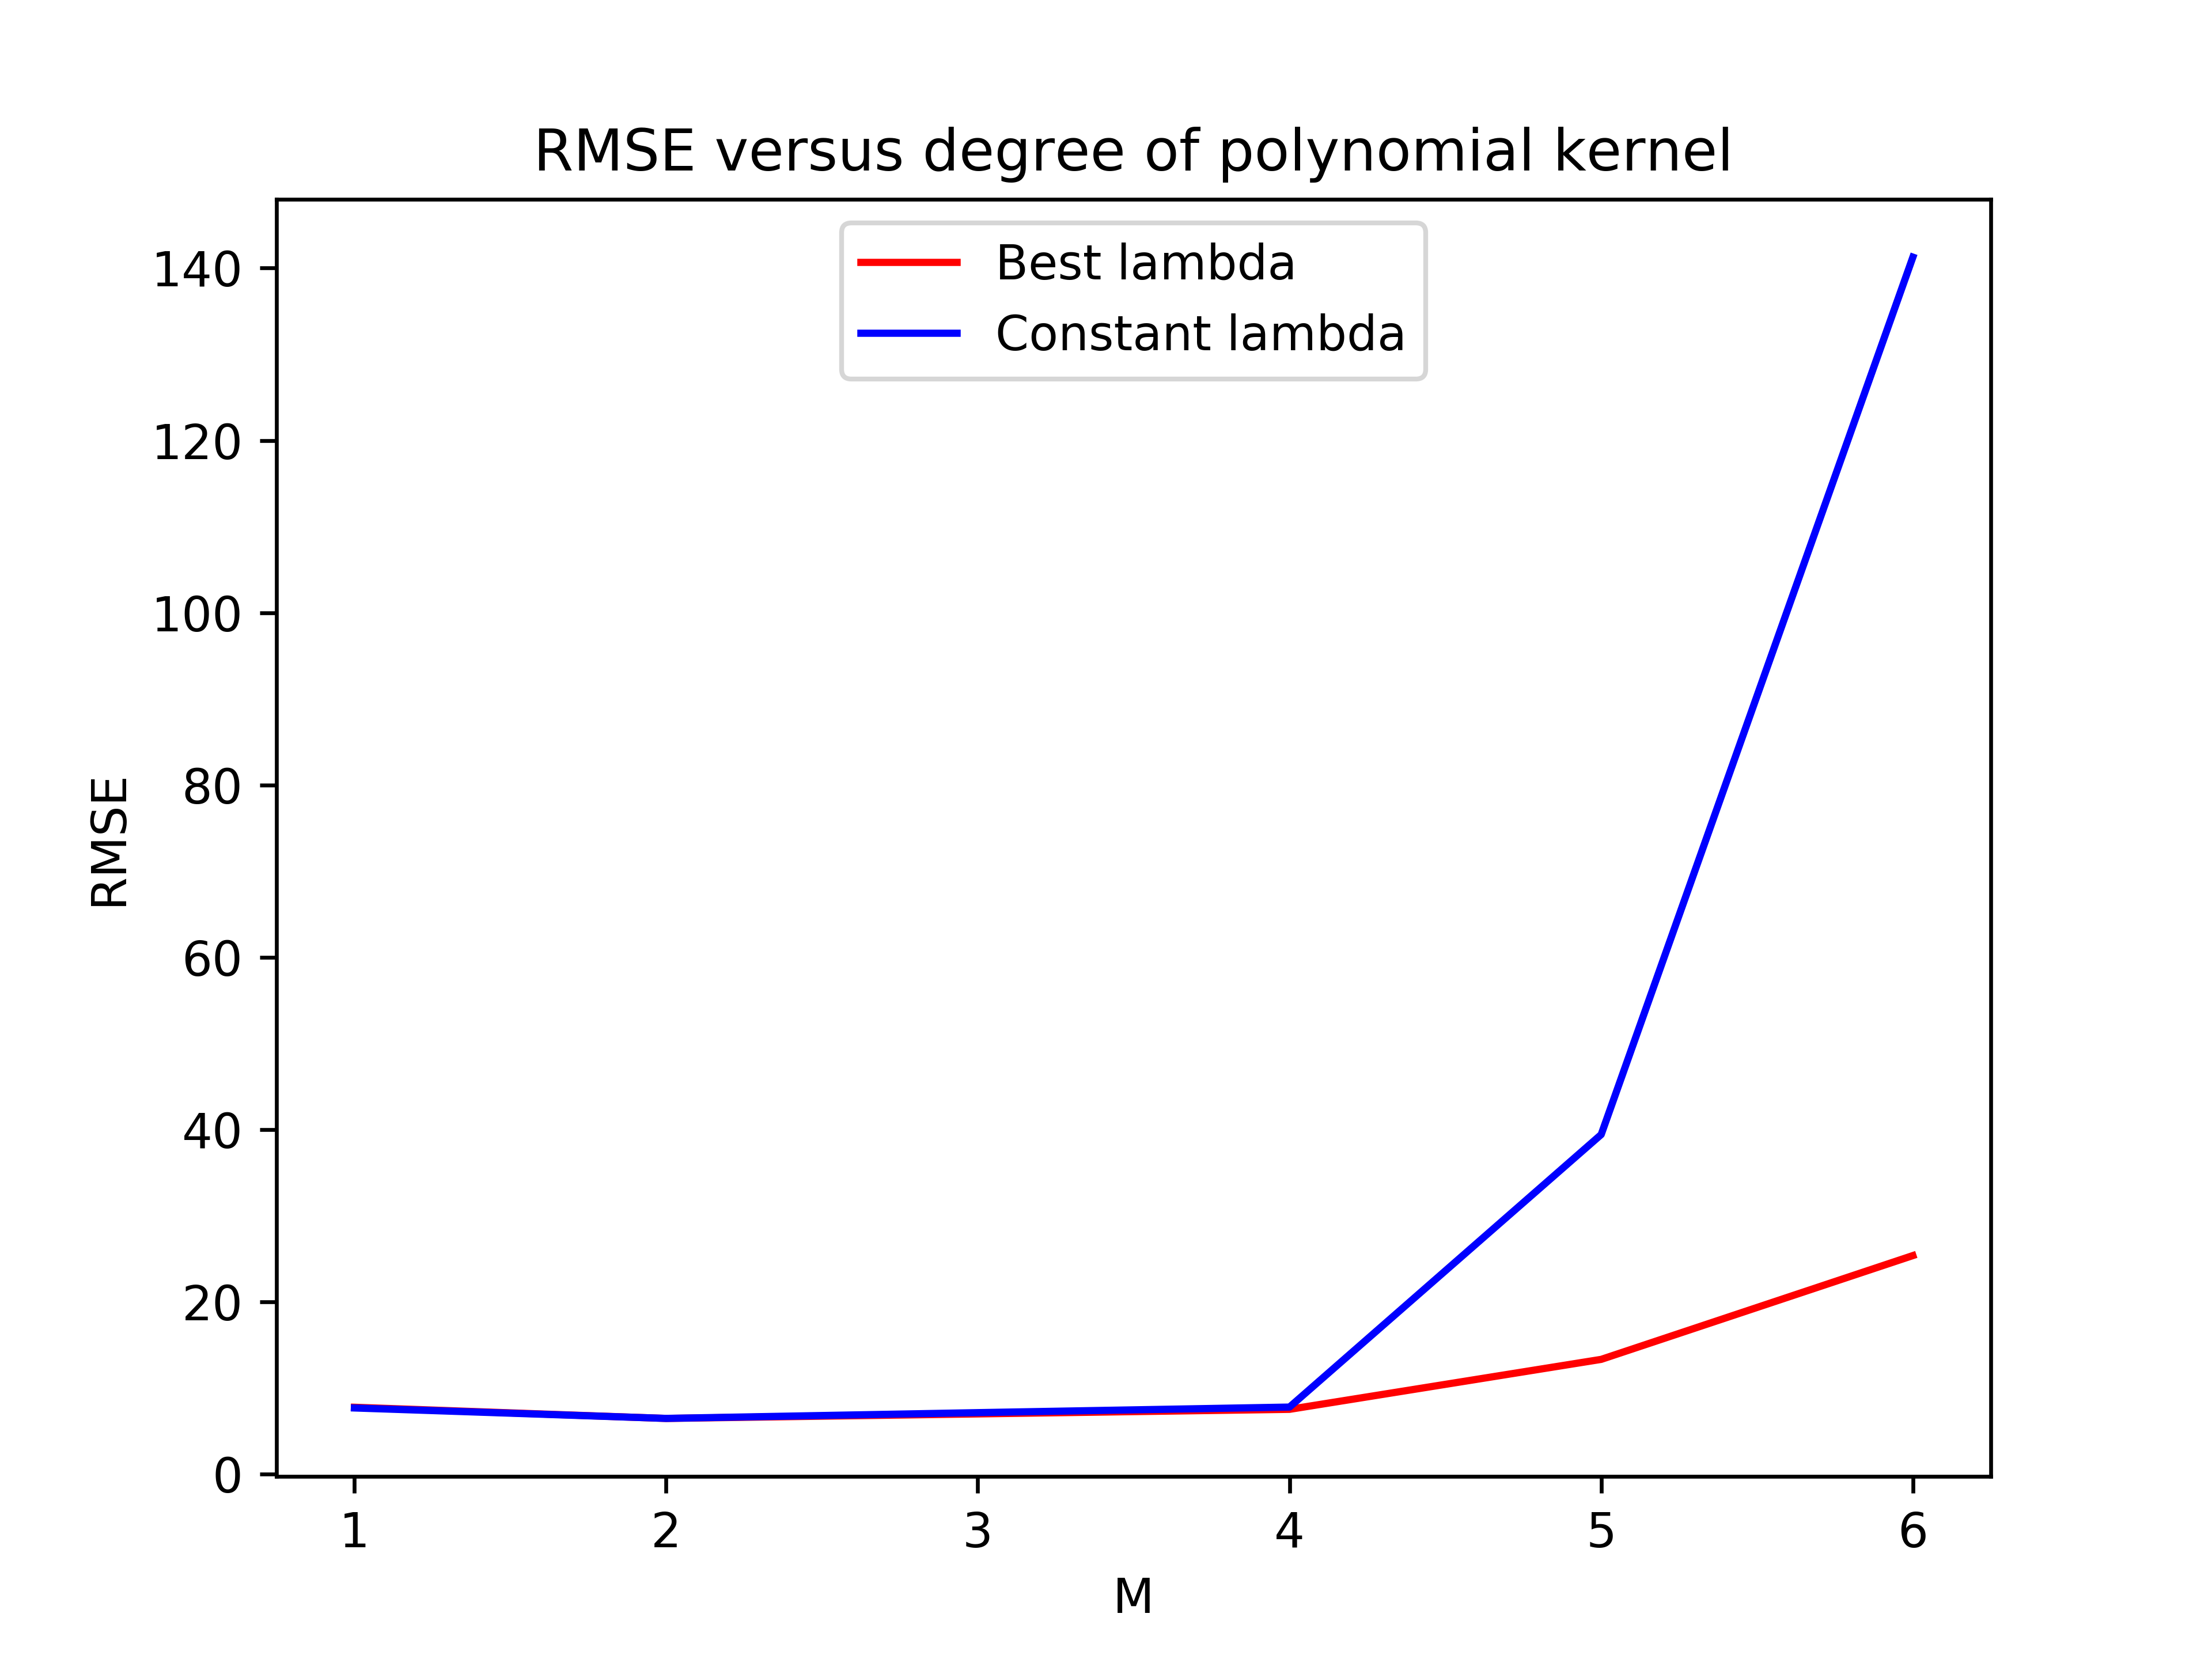
\includegraphics[width=.4\textwidth]{housing_pol.png}
    \caption{Polynomial kernel}
    \label{fig:house_pol}
\end{figure}

\begin{figure}[ht]
    \centering
    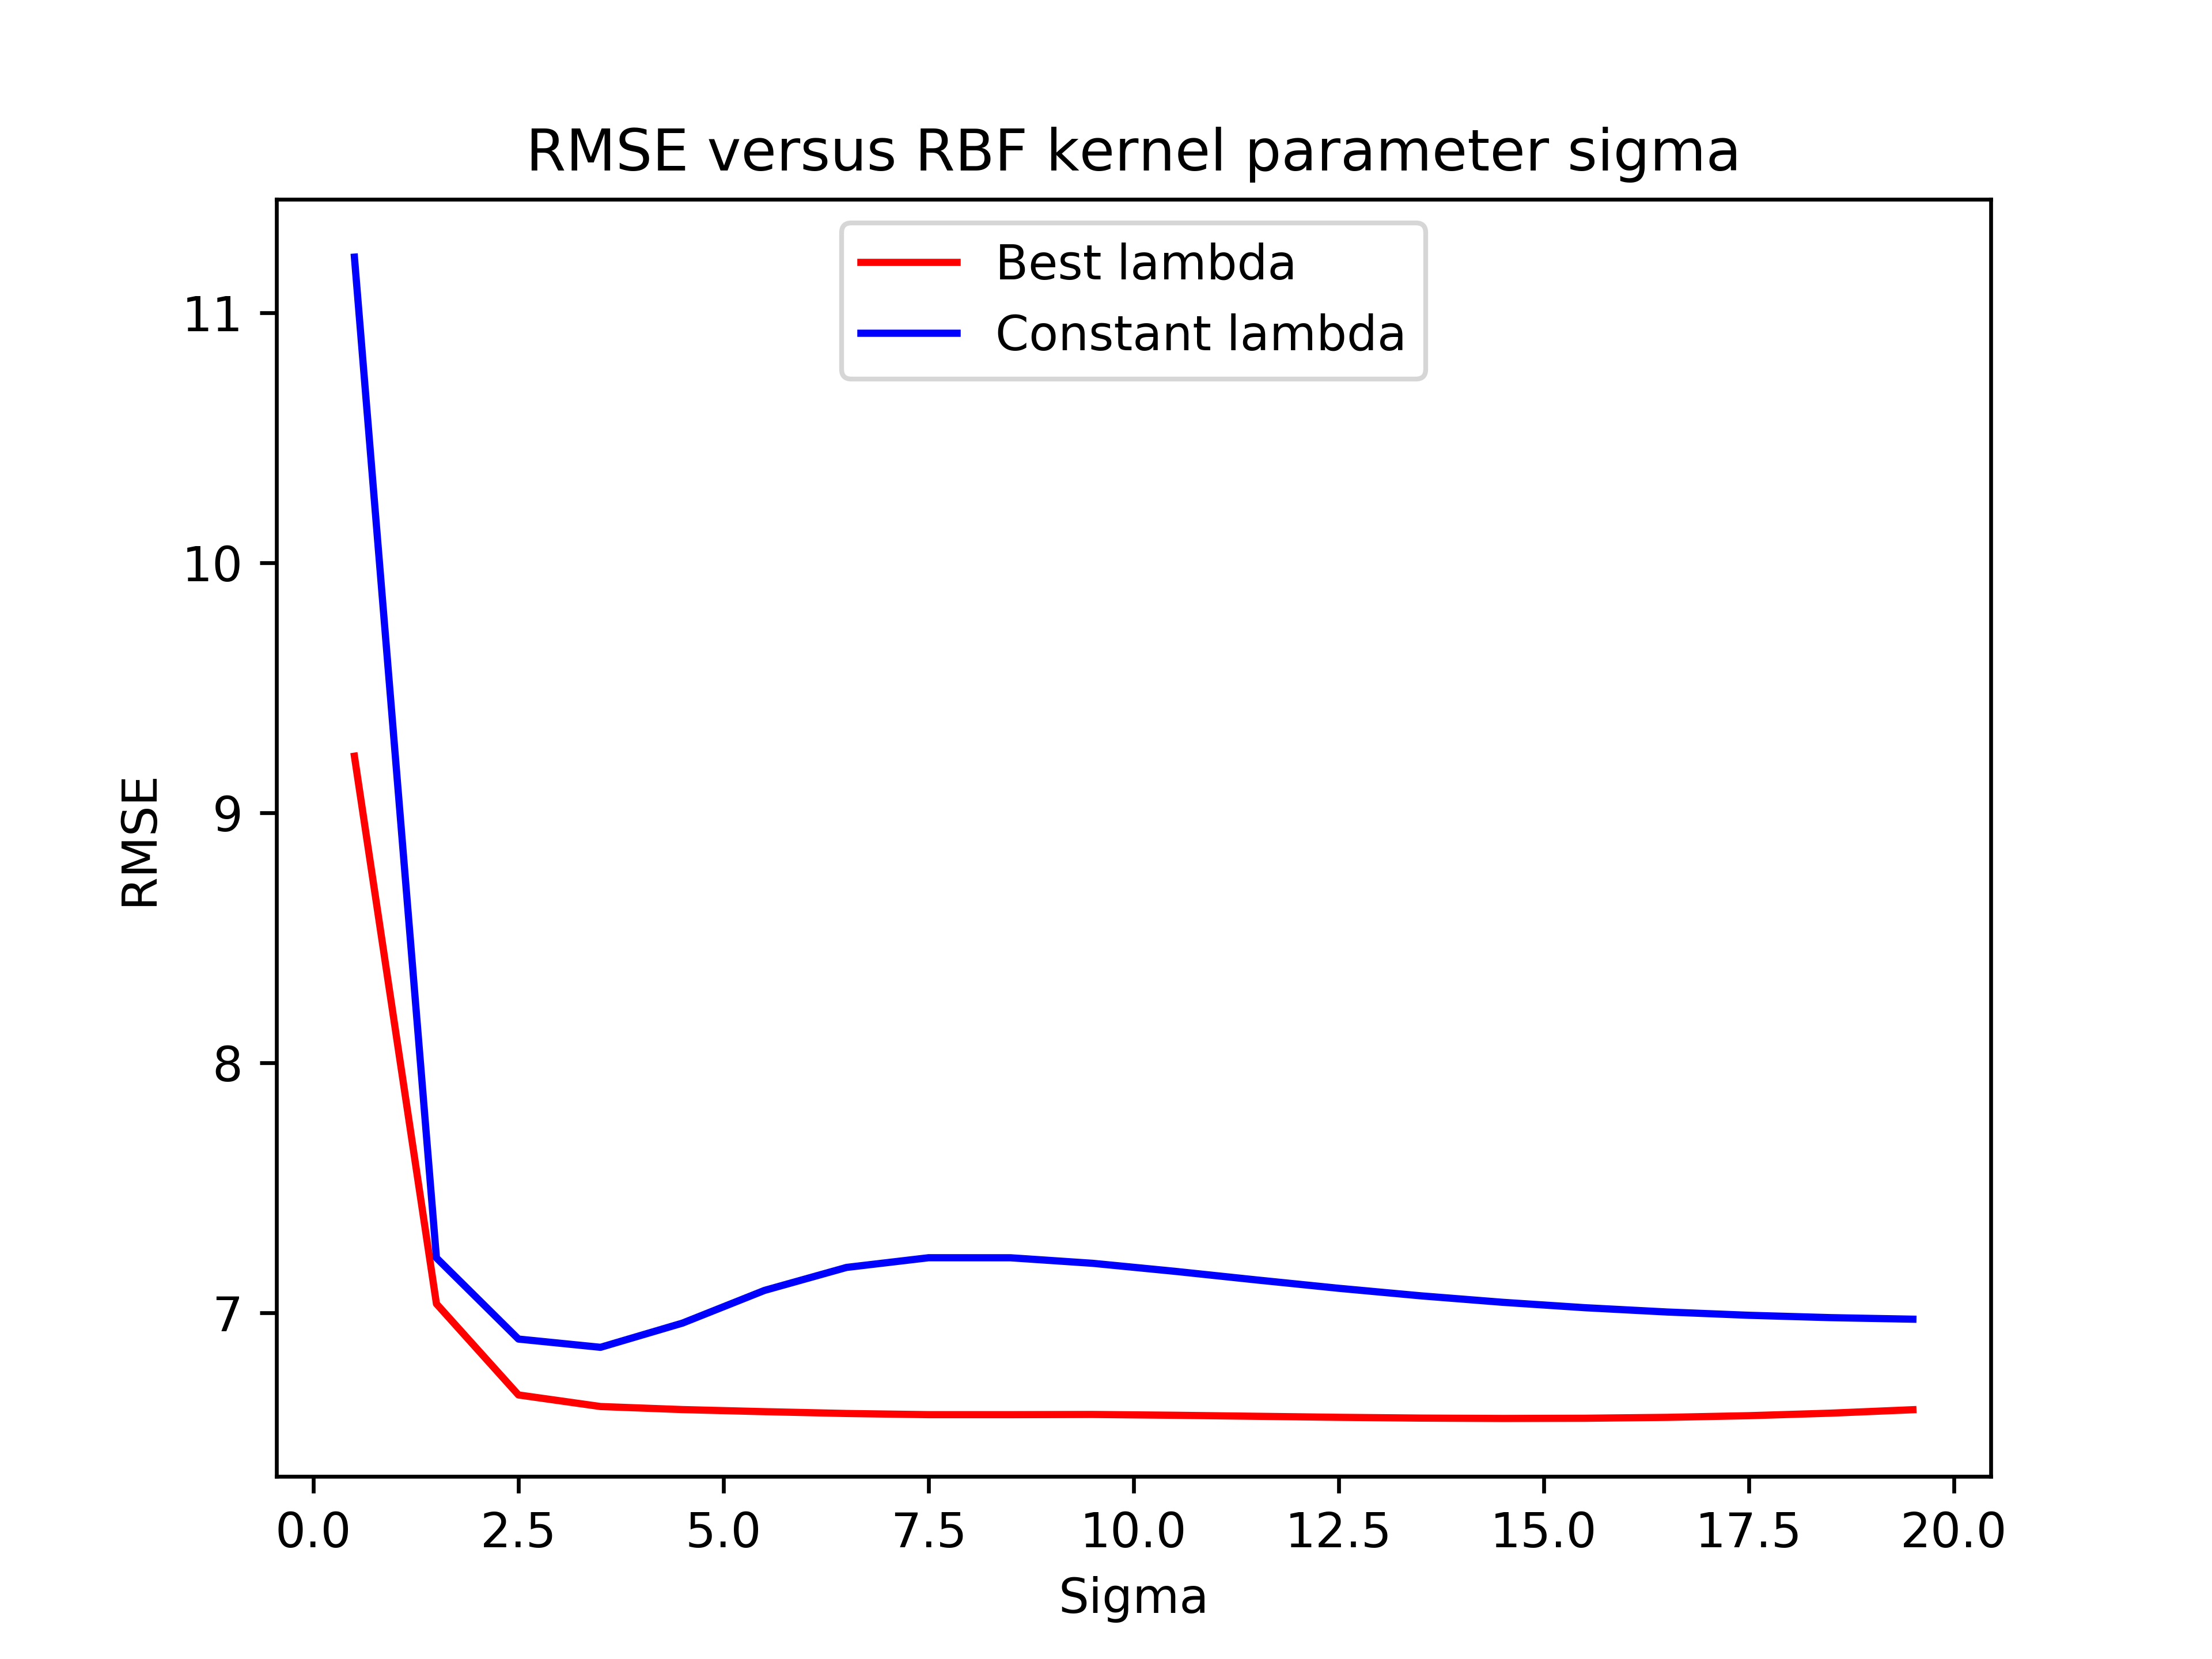
\includegraphics[width=.4\textwidth]{housing_rbf.png}
    \caption{RBF kernel}
    \label{fig:house_rbf}
\end{figure}

\end{document}